 \documentclass[12pt]{article}
\usepackage{amsmath}
\usepackage{amssymb}
\usepackage{geometry}
\usepackage{amsmath, amsfonts, bm, graphicx}
\usepackage{tabularx}
\usepackage{booktabs} 
\usepackage{float}
\usepackage{enumitem,cancel}
\geometry{margin=1in}


\title{}
\date{}
\author{}
\DeclareMathOperator{\Real}{Re}
\DeclareMathOperator{\Imag}{Im}

\begin{document}
\subsection*{\boxed{\text{HW 8 - Zeshui Song}}}
\underline{Notes:}
\begin{itemize}
    \item A sinusoidal forcing function always results in a sinusoidal forced response of the same frequency in a linear circuit. This means that if the input is a sine then the output is a sine of the same frequency, but possibly different amplitude and phase. 
    \item We can rewrite sinusoidal functions as the real and imaginary part of a complex exponential through Euler's identity
    \[e^{j\omega t} = \cos(\omega t) + j\sin(\omega t)\]
    \[cos(\omega t + \phi) = \Real\{e^{j(\omega t + \phi)}\}\]
    \[\sin(\omega t + \theta) = \Imag\{e^{j(\omega t + \theta)}\}\]
    \item Since all sinusoidal functions have the same frequency, we can use phasor notation, supressing the time dependence term $e^{j\omega t}$, resulting in a phasor.
   \begin{center}
    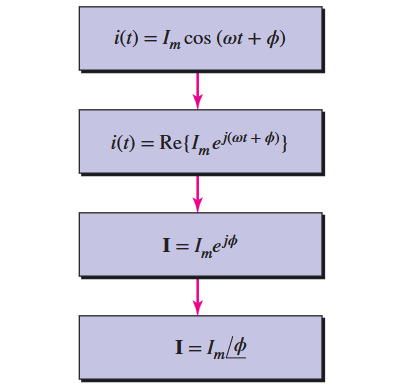
\includegraphics[width=0.4\textwidth]{Phasor transform.png}
   \end{center}
   Note that $\mathbf{I}$ represent complex numbers, and we will take the real or imaginary part of the resulting phasor to get to the actual time domain response.\\\\
   Additionally, differentiation and integration in the time domain correspond to multiplication and division by $j\omega$ in the phasor domain, respectively.
   \newpage
   \item $\mathbf{V}$ and $\mathbf{I}$ relationships:
   \begin{center}
    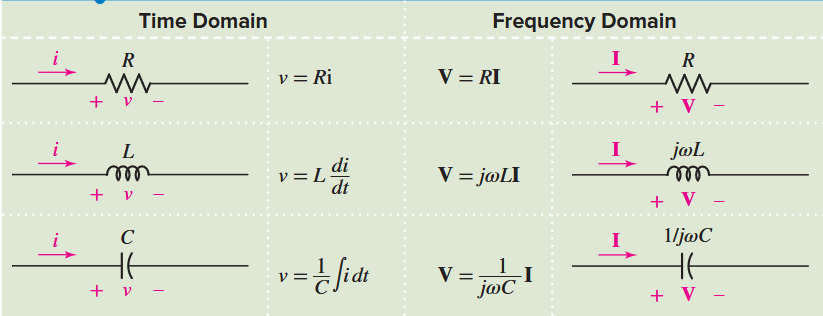
\includegraphics[width=0.8\textwidth]{VI.png}
   \end{center}
   We can use these complex valued currents and voltages with KCL and KVL as we normally would to analyze circuits, and then take the real or imaginary part of the resulting phasor to get to the actual time domain response.
   \item We define \textbf{impedance} to be the relationship between the complex voltage and current in a circuit element:
   \[\mathbf{Z} = \frac{\mathbf{V}}{\mathbf{I}}\]
   These impedances sum in series and parallel just like resistances and can also be used in nodal and mesh analysis using the relationship $\mathbf{V} = \mathbf{IZ}$ (just like Ohm's law).
   \item Since $\mathbf{Z}$ is a complex number, we can express it either in rectangular form $\mathbf{Z} = R + jX$ or in polar form $\mathbf{Z} = |\mathbf{Z}|e^{j\theta}$, where $R$ is the real part of the impedance (resistance), and $X$ is the imaginary part of the impedance (reactance).  
   \item Although we have complex voltages and currents for sinusoidal sources, because the circuit is linear, \textbf{superposition}, \textbf{source transformations}, and \textbf{Thevenin/Norton equivalents} still apply in the phasor domain. Just remember to use impedances instead of resistances.
\end{itemize}

\newpage
\section*{10.2}
\vspace{-2em}
\begin{center}
    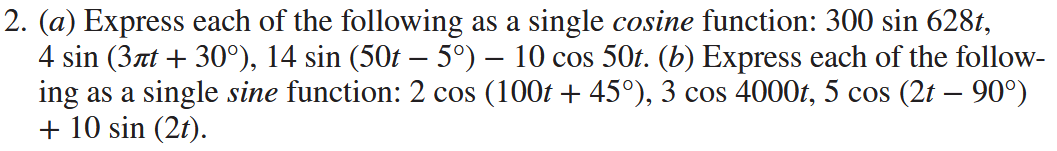
\includegraphics[width=0.8\textwidth]{10-2.png}
\end{center}
We can rewrite this as a single cosine using the trig identities:
\[\boxed{\sin(\theta) = \cos(\theta - 90^\circ),\quad \cos(\theta) = \sin(\theta + 90^\circ)}\]
Note that while it is true that $\sin(\theta) = \cos(90^\circ - \theta)$ and $\cos(\theta) = \sin(90^\circ - \theta)$, the negative sign on $\theta$ would change the direction of the phasor from CCW to CW, so to keep consistency, we will try to keep $\theta$ positive.\\\\
\textbf{(a)} $300\sin(628t)$\\
\[\boxed{300\sin(628t)=300\cos(628t - 90^\circ)}\]
\textbf{(b)} $4\sin(3\pi t +30^\circ)$
\[\boxed{4\sin(3\pi t +30^\circ)=4\cos(3\pi t - 60^\circ)}\]
\textbf{(c)} $14\sin(50t-5^\circ)-10\cos(50t)$\\\\
Here it would be useful to perform this addition using phasors. First converting each term to a cosine:
\[14\sin(50t-5^\circ)=14\cos(50t - 95^\circ)\]
Both have the same frequency, so we can represent them as phasors and add them:
\[14\cos(50t - 95^\circ) = 14\angle -95^\circ,\quad -10\cos(50t) = -10\angle 0^\circ\]
\begin{center}
    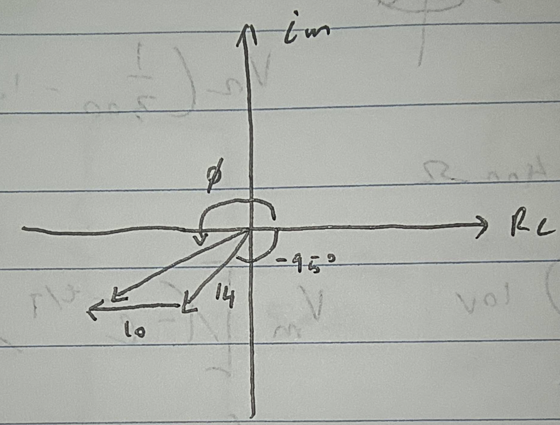
\includegraphics[width=0.4\textwidth]{10-2-1.png}
\end{center}
The sum has magnitude 
\[\sqrt{(14\cos(-95^\circ)-10)^2+(14\sin(-95^\circ))^2}=17.899\]
and angle
\[\tan^{-1}\left(\frac{14\sin(-95^\circ)}{(14\cos(-95^\circ)-10)}\right)=51.183^\circ\]
Since $tan^{-1}$ only gives $-90^\circ$ to $90^\circ$, we need to add $180^\circ$ to get the correct angle 
\[\phi = 51.183^\circ + 180^\circ = 231.183^\circ\]
Thus the sum is
\[14\cos(50t - 95^\circ)-10\cos(50t)=\Real(17.899e^{j(50t+231.183^\circ)})=\boxed{17.899\cos(50t + 231.183^\circ)}\]
\textbf{(d)} $2\cos(100t+45^\circ)$ as a sine:
\[\boxed{2\cos(100t+45^\circ)=2\sin(100t + 135^\circ)}\]
\textbf{(e)} $3\cos(4000t)$
\[\boxed{3\cos(4000t)=3\sin(4000t + 90^\circ)}\]
\textbf{(f)} $5\cos(2t-90^\circ)+10\sin(2t)$\\\\
First we convert to phasors, using sin as our reference (the positive imaginary axis is now $0^\circ$):
\[5\cos(2t-90^\circ) = 5\sin(2t)=5\angle 0^\circ,\quad 10\sin(2t) = 10\angle 0^\circ\]
\begin{center}
    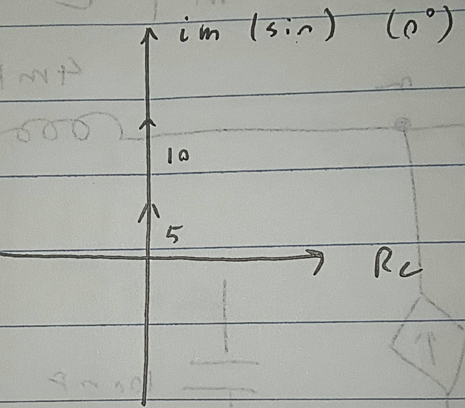
\includegraphics[width=0.4\textwidth]{10-2-2.png}
\end{center}
The sum has magnitude
\[\sqrt{(5+10)^2} = 15\]
and angle
\[\tan^{-1}\left(\frac{0}{5+10}\right) = 0^\circ\]
Thus the sum is
\[5\sin(2t)+10\sin(2t)=\Imag(15e^{j(2t+0^\circ)})=\boxed{15\sin(2t)}\]

\section*{10.9}
\vspace{-2em}
\begin{center}
    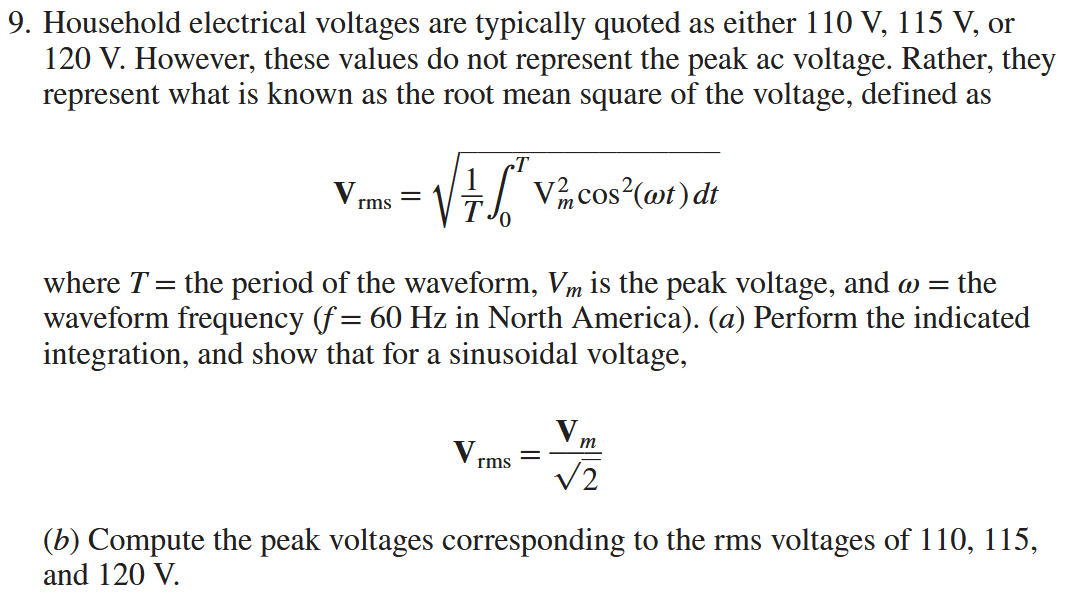
\includegraphics[width=0.8\textwidth]{10-9.png}
\end{center}
Note that while the values are given in the frequency domain (denoted by the bold $\mathbf{V}$), the exponential term $e^{j\phi}$ is constant through time so its just a constant that sticks around.\\\\
\textbf{(a)} First evaluating the inside integral:
\[\frac{1}{T}\int_{0}^{T} V_m^2\cos^2(\omega t)\,dt=\frac{V_m^2}{T}\int_{0}^{T} \cos^2(\omega t)\,dt\]
\[\int_{0}^{T} \cos^2(\omega t)\,dt = \int_{0}^{T} \frac{\cos(2\omega t)+1}{2}\,dt = \left[\frac{t}{2}\right]_{0}^{T}+\left[\frac{\sin(2\omega t)}{4\omega}\right]_{0}^{T} = \frac{T}{2}+0\]
\underline{Note:} The $\sin(2\omega t)$ term is $0$ because $\omega = \frac{2\pi}{T}$, so $2\omega T = 4\pi$, and $\sin(4\pi) = 0$.\\\\
Thus:
\[\mathbf{V}_{rms} = \sqrt{\frac{V_m^2}{T}\frac{T}{2}} = \boxed{\frac{V_m}{\sqrt{2}}}\]
\textbf{(b)} To find the peak voltages ($\mathbf{V_m}$), we just need to apply to rms formula:
\[\mathbf{V_m} = \mathbf{V}_{rms} \cdot \sqrt{2}\]
\begin{itemize}
    \item $110V$ rms $\Rightarrow 155.56V$ peak
    \item $115V$ rms $\Rightarrow 162.63V$ peak
    \item $120V$ rms $\Rightarrow 169.71V$ peak
\end{itemize}

\section*{10.11}
\vspace{-2em}
\begin{center}
    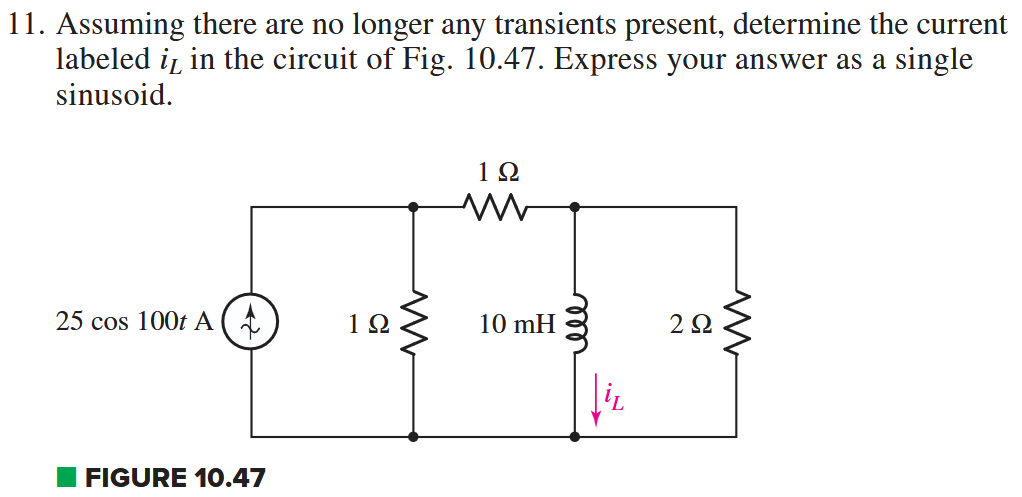
\includegraphics[width=0.8\textwidth]{10-11.png}
\end{center}
Since this circuit is at sinusoidal steady state, we can use phasor analysis with impedances to solve the problem ($\mathbf{V} = \mathbf{IZ}$).\\\\
First, using a source transformation to turn the current source into a voltage source:
\[\mathbf{I_s}=25\angle 0^\circ,\quad R_p = 1\,\Omega\]
\[\implies \mathbf{V_s} = \mathbf{I_s} \cdot R_p = 25\angle 0^\circ \cdot [1\,\Omega] = 25\angle 0^\circ\]
Combining the 1$\Omega$ and 1$\Omega$ resistors in series:
\begin{center}
    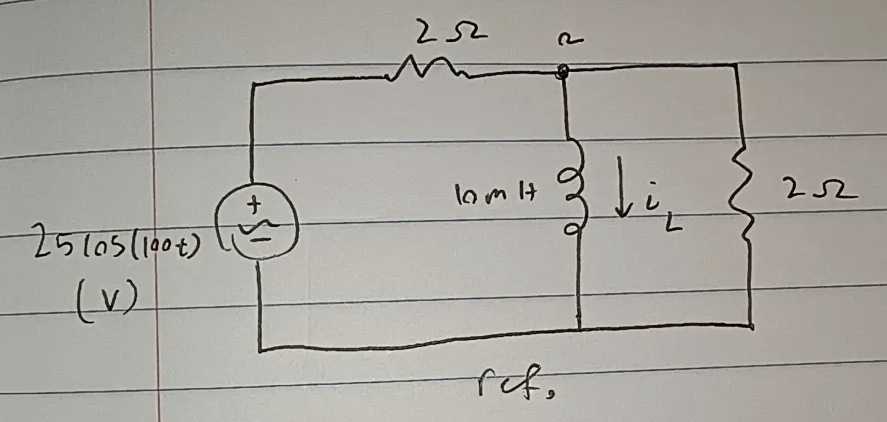
\includegraphics[width=0.8\textwidth]{10-11-1.png}
\end{center}
Using nodal analysis (KCL) at the top node:
\[\frac{\mathbf{V_s}-\mathbf{V_a}}{[2\,\Omega]}=\frac{\mathbf{V_a}}{j[100\,\text{rad/s}]\cdot[10\times10^{-3}\,\text{H}]}+\frac{\mathbf{V_a}}{[2\,\Omega]}\]
In rectangular form, $\mathbf{V_s} = 25 + j0$, and $j[100\,\text{rad/s}]\cdot[10\times10^{-3}\,\text{H}] = 1j$. Thus:
\[\frac{(25)-\mathbf{V_a}}{2}=\frac{\mathbf{V_a}}{1j}+\frac{\mathbf{V_a}}{2}\]
Solving for $\mathbf{V_a}$:
\[\mathbf{V_a}(1-j) = \frac{25}{2}\]
\underline{Note:} $1/j = -j$, we see this by multiplying by $j/j$.
\[\mathbf{V_a} = \frac{25}{2(1-j)} = \frac{25}{2} \cdot \frac{1+j}{(1-j)(1+j)} = \frac{25}{2} \cdot \frac{1+j}{1+1} = \frac{25}{4}(1+j)\]
\[\mathbf{V_a} = 6.25 + 6.25j\]
\underline{Note:} Remember that rectangular form and polar form are equivalent ways of representing phasors. Typically rectangular form is easier for addition and subtraction (sum components), while polar form is easier for multiplication and division (add angles and multiply magnitudes).\\\\
Now to find the current through the inductor, we can use $\mathbf{V} = \mathbf{IZ}$:
\[\mathbf{I_L}=\frac{\mathbf{V_a}}{j1}=\frac{6.25 + j6.25}{j}=-6.25j+6.25\,[\text{A}]\]
Now we can convert from phasor form back to the time domain:\\
\begin{minipage}[t]{0.3\textwidth}
\vspace{0pt}
\centering
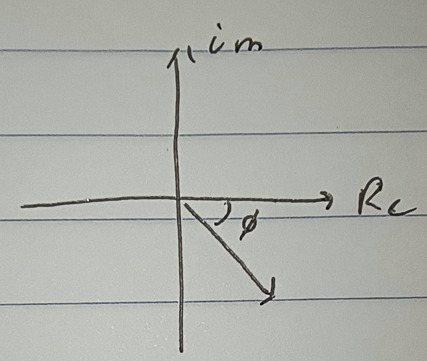
\includegraphics[width=\textwidth]{10-11-2.png}
\end{minipage}
\hfill
\begin{minipage}[t]{0.6\textwidth}
\vspace{0pt}
\[|\mathbf{I_L}|=\sqrt{6.25^2+(-6.25)^2}=8.838\]
\[\phi = \tan^{-1}\left(\frac{-6.25}{6.25}\right) = -45^\circ\]
\[\mathbf{I_L} = 8.838\angle -45^\circ = \boxed{8.838\sin(100t - 45^\circ)\,\text{[A]}}\]
\end{minipage}
\newpage

\section*{10.23}
\vspace{-2em}
\begin{center}
    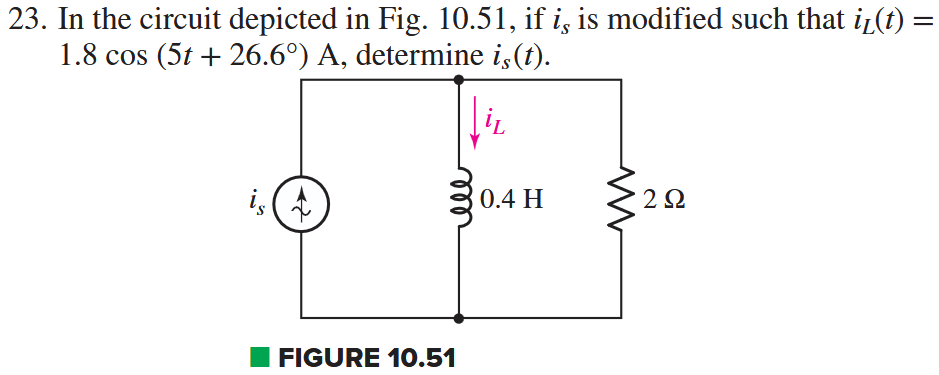
\includegraphics[width=0.8\textwidth]{10-23.png}
\end{center}
Given the current through the inductor, we can apply current division to solve for $\mathbf{I_s}$:
\[\mathbf{I_L} = 1.8\angle 26.6^\circ = 1.609+j0.805\]
Current division says:
\[\mathbf{I_L} = \frac{\frac{1}{\mathbf{Z_L}}}{\frac{1}{\mathbf{Z_L}}+\frac{1}{R}}\mathbf{I_s}=\frac{R}{\mathbf{Z_L}+R}\mathbf{I_s}\]
\[\implies \mathbf{I_s} = \frac{\mathbf{Z_L}+R}{R}\mathbf{I_L}\]
Note that $\mathbf{Z_L} = j\omega L = j[5\,\text{rad/s}]\cdot[0.4\,\text{H}] = 2j$. Thus:
\[\mathbf{I_s} = \frac{2j+2}{2}\mathbf{I_L}\]
Since its easier to do multiplication and division in polar form, we can convert the first term to polar form:
\[\frac{2j+2}{2} = 1+j\]
Magnitude: $\sqrt{(1)^2+(1)^2}=1.4142$\\\\
Angle: $\tan^{-1}\left(\frac{1}{1}\right)=45^\circ$\\\\
Thus:
\[\mathbf{I_s} = \frac{\mathbf{Z_L}+R}{R}\mathbf{I_L} = (1.4142\angle 45^\circ)\cdot(1.8\angle 26.6^\circ)\]
\[\mathbf{I_L} = 2.545\angle 71.6^\circ\]
Converting back to time domain:
\[\boxed{\mathbf{I_L} = 2.545\cos(5t + 71.6^\circ)}\]
\underline{Note:} Since the resulting current is a cosine, the forcing function must also be a cosine. So just adding back the time dependence term $e^{j\omega t}$, and taking the real part, we get our solution.

\section*{10.35}
\vspace{-2em}
\begin{center}
    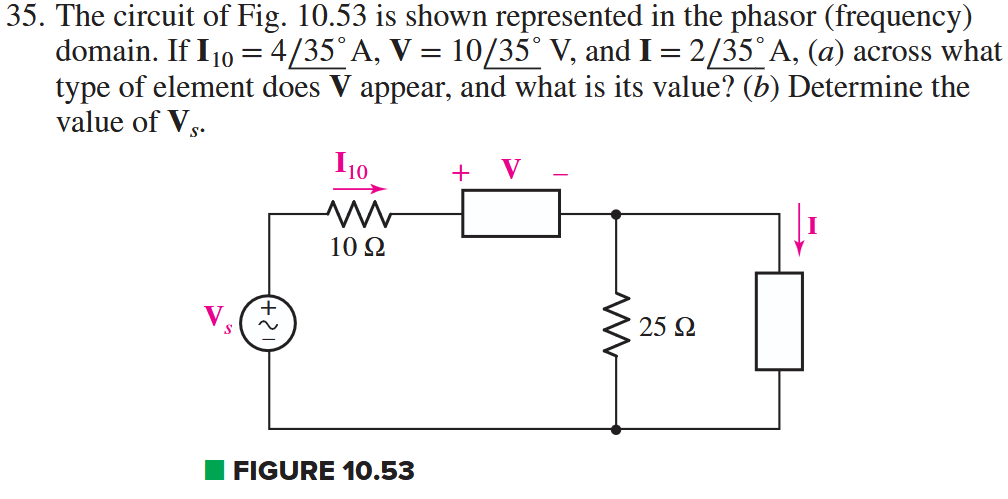
\includegraphics[width=0.8\textwidth]{10-35.png}
\end{center}
\textbf{(a)} To find the impedance of the element corresponding to $\mathbf{V}$, we can use the relationship $\mathbf{V} = \mathbf{IZ}$:
\[\mathbf{Z} = \frac{\mathbf{V}}{\mathbf{I}} = \frac{(10\angle 35^\circ)}{(4\angle 35^\circ)} = 2.5\angle 0^\circ \]
Since it has a phase angle of $0^\circ$, this means that the element is purely resistive (no imaginary term, so no reactance). Thus the element is a $2.5\,\Omega$ resistor.\\\\
\textbf{(b)} To find $\mathbf{V_s}$, we can use KCL at the top node to find the current entering the 25 $\Omega$ resistor, and then use $\mathbf{V} = \mathbf{IZ}$ to find the voltage across the 25 $\Omega$ resistor. Then, we can use KVL around the left loop to find $\mathbf{V_s}$:
\[\mathbf{I_{10}} = \mathbf{I_{25}} + \mathbf{I}\]
\[\implies \mathbf{I_{25}} = \mathbf{I_{10}} - \mathbf{I} = (4\angle 35^\circ) - (2\angle 35^\circ) = 2\angle 35^\circ\]
\[\mathbf{V_{25}} = \mathbf{I_{25}} \cdot [25\,\Omega] = (2\angle 35^\circ)\cdot(25\,\Omega) = 50\angle 35^\circ\]
KVL:
\[\mathbf{V_s}-\mathbf{I_{10}}\cdot[10\,\Omega] - \mathbf{V} - \mathbf{I_{25}}\cdot[25\,\Omega] = 0\]
\[\mathbf{V_s} = (4\angle 35^\circ)\cdot(10\,\Omega) + (10\angle 35^\circ) + (50\angle 35^\circ) = \boxed{100\angle 35^\circ}\]
\newpage

\section*{10.41}
\vspace{-2em}
\begin{center}
    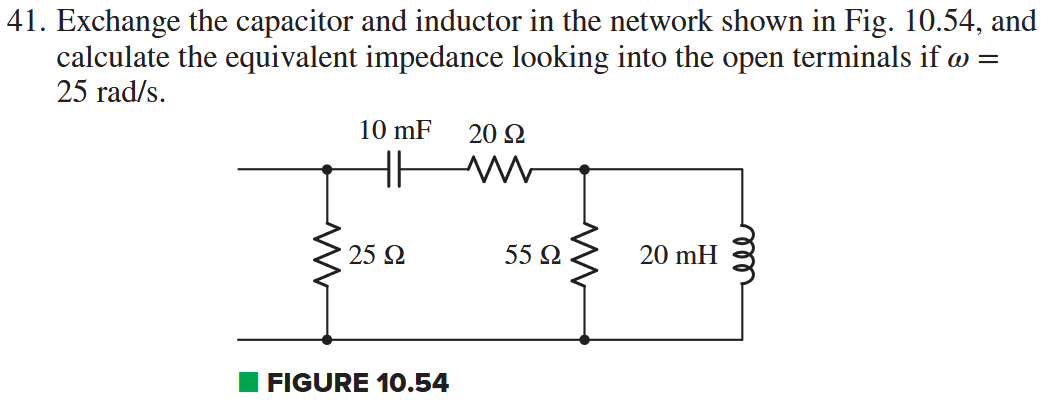
\includegraphics[width=0.8\textwidth]{10-41.png}
\end{center}
First redraw the circuit having exchanged the capacitor and inductor:
\begin{center}
    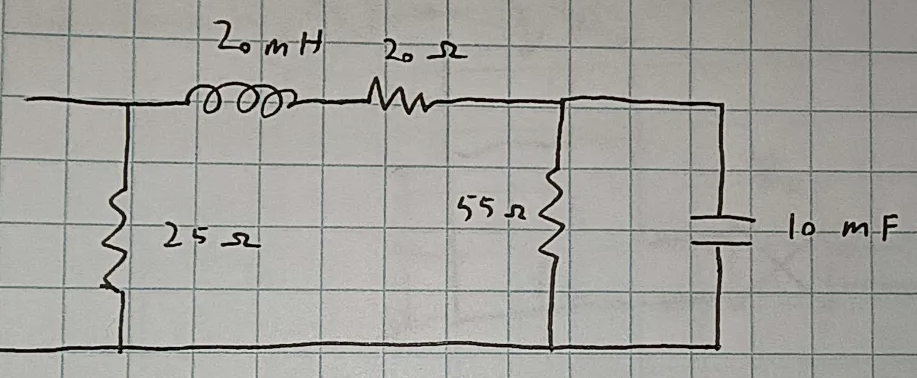
\includegraphics[width=0.8\textwidth]{10-41-1.png}
\end{center}
Sum the 55 $\Omega$ resistor in parallel with the 10 mF capacitor:
\[\frac{1}{j\omega C} = \frac{1}{j[25\,\text{rad/s}]\cdot[10\times10^{-3}\,\text{F}]} = \frac{1}{0.25j} = -4j\]
\[\mathbf{Z} = \frac{(-4j)[55\,\Omega]}{(-4j) + [55\,\Omega]} = \frac{-220j}{55-4j}=\frac{-220j(55+4j)}{(55-4j)(55+4j)}\]
\[\mathbf{Z} = \frac{-12100j+880}{3041} = 0.289-3.978j\]
Sum the 20 mH inductor in series with the 20 $\Omega$ resistor and $\mathbf{Z}$:
\[j\omega L = j[25\,\text{rad/s}]\cdot[20\times10^{-3}\,\text{H}] = 0.5j\]
\[\mathbf{Z_1} = (0.5j) + [20\,\Omega] + \mathbf{Z} = 0.5j+20+0.289-3.978j\]
\[\mathbf{Z_1} = 20.289-3.478j\]
Finally, we can sum $\mathbf{Z_1}$ in parallel with the 25 $\Omega$ resistor:
\[\mathbf{Z_\text{eq}} = \frac{\mathbf{Z_1}\cdot[25\,\Omega]}{\mathbf{Z_1} + [25\,\Omega]} = \frac{(20.289-3.478j)(25)}{20.289-3.478j + 25}\]
\[\mathbf{Z_\text{eq}} = \frac{507.225-86.95j}{45.289-3.478j}\]
We can divide in polar form more easily, so we can convert the numerator and denominator to polar form:
\[\sqrt{(507.225)^2+(-86.95)^2} = 514.62, \quad \tan^{-1}\left(\frac{-86.95}{507.225}\right) = -9.727^\circ\quad \text{(numerator)}\]
\[\sqrt{(45.289)^2+(-3.478)^2} = 45.42, \quad \tan^{-1}\left(\frac{-3.478}{45.289}\right) = -4.39^\circ\quad \text{(denominator)}\]
\[\mathbf{Z_\text{eq}} = \frac{514.62\angle -9.727^\circ}{45.42\angle -4.39^\circ} = \boxed{11.33\angle -5.33^\circ}\]

\section*{10.44}
\vspace{-2em}
\begin{center}
    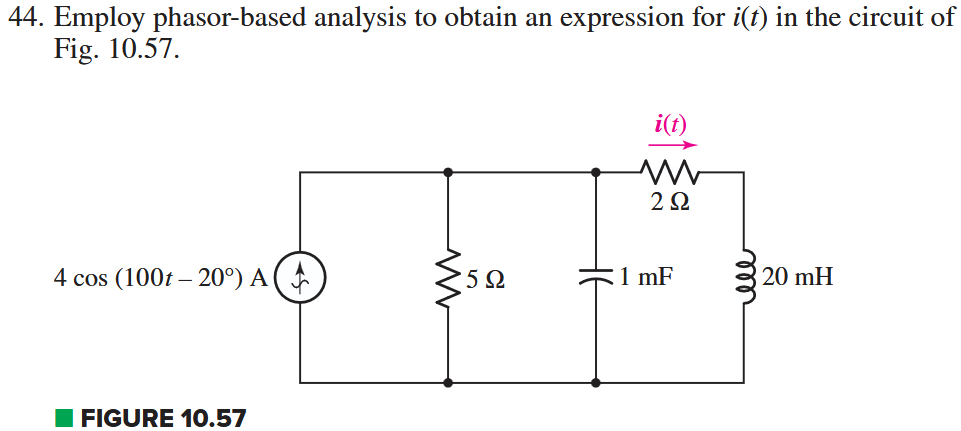
\includegraphics[width=0.8\textwidth]{10-44.png}
\end{center}
Source:
\[\mathbf{I_s} = 4\angle -20^\circ\]
Source transformation: $R_p = 5\,\Omega$:
\[\mathbf{V_s} = \mathbf{I_s} \cdot R_p = (4\angle -20^\circ)\cdot[5\,\Omega] = 20\angle -20^\circ\]
\[\mathbf{V_s} = 18.793-6.84j\]
Redrawing the circuit:
\begin{center}
    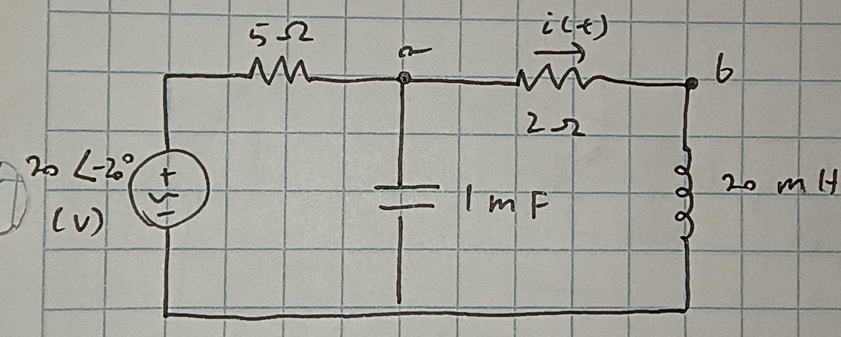
\includegraphics[width=0.8\textwidth]{10-44-1.png}
\end{center}
Nodal analysis at node a:
\[\frac{1}{j\omega C} = \frac{1}{j[100\,\text{rad/s}]\cdot[10^{-3}\,\text{F}]} = \frac{1}{0.1j} = -10j\]
\[j\omega L = j[100\,\text{rad/s}]\cdot[20\times10^{-3}\,\text{H}] = 2j\]
\[\frac{(18.793-6.84j)-\mathbf{V_a}}{[5\,\Omega]} = \frac{\mathbf{V_a}}{-10j} +\frac{\mathbf{V_a}-\mathbf{V_b}}{[2\,\Omega]}\]
\[\implies 3.758-1.368j = (0.7+0.1j)\mathbf{V_a}-0.5\mathbf{V_b}\]
Nodal analysis at node b:
\[\frac{\mathbf{V_a}-\mathbf{V_b}}{[2\,\Omega]}=\frac{\mathbf{V_b}}{2j}\]
\[\implies 0 = 0.5\mathbf{V_a} + (-0.5+0.5j)\mathbf{V_b}\]
\[\mathbf{V_b} = \frac{-0.5}{(-0.5+0.5j)}\mathbf{V_a}\]
Plugging into the first equation and solving for $\mathbf{V_a}$:
\[\begin{aligned}
    3.758-1.368j &= (0.7+0.1j)\mathbf{V_a}-0.5\frac{-0.5}{(-0.5+0.5j)}\mathbf{V_a}\\
3.758-1.368j &= (0.7+0.1j)\mathbf{V_a}+\frac{0.25(-0.5-0.5j)}{(-0.5+0.5j)(-0.5-0.5j)}\mathbf{V_a}\\
3.758-1.368j &= (0.7+0.1j)\mathbf{V_a}+\frac{-0.125-0.125j}{0.25+0.25}\mathbf{V_a}\\
3.758-1.368j &= (0.7+0.1j)\mathbf{V_a}+(-0.25-0.25j)\mathbf{V_a}\\
3.758-1.368j &= (0.45-0.15j)\mathbf{V_a}
\end{aligned}\]
\[\implies \mathbf{V_a} = \frac{3.758-1.368j}{0.45-0.15j}\]
Using polar form to divide:
\[\sqrt{(3.758)^2+(-1.368)^2} = 3.99, \quad \tan^{-1}\left(\frac{-1.368}{3.758}\right) = -20.00^\circ\quad \text{(numerator)}\]
\[\sqrt{(0.45)^2+(-0.15)^2} = 0.474, \quad \tan^{-1}\left(\frac{-0.15}{0.45}\right) = -18.43^\circ\quad \text{(denominator)}\]
\[\mathbf{V_a} = \frac{3.99\angle -20.00^\circ}{0.474\angle -18.43^\circ} = 8.417\angle -1.57^\circ\]
Plug back into the second equation to find $\mathbf{V_b}$:
\[\mathbf{V_b} = \frac{-0.5}{(-0.5+0.5j)}\mathbf{V_a}=\frac{-1}{(-1+j)}\mathbf{V_a}=\frac{-1(-1-j)}{(-1+j)(-1-j)}\mathbf{V_a}\]
\[\mathbf{V_b} = \frac{1+j}{2}\mathbf{V_a}\]
Convert to polar form to multiply:
\[0.5+0.5j = 0.707\angle 45^\circ\]
\[\mathbf{V_b} = (0.707\angle 45^\circ)(8.417\angle -1.57^\circ) = 5.95\angle 43.43^\circ\]
Finally, we can find the current through the 2 $\Omega$ resistor using $\mathbf{V} = \mathbf{IZ}$:
\[\mathbf{I} = \frac{\mathbf{V_a}-\mathbf{V_b}}{[2\,\Omega]}=\frac{(8.417\angle -1.57^\circ)-(5.95\angle 43.43^\circ)}{2}\]
Convert to rectangular form to subtract:
\[8.417\angle -1.57^\circ = 8.417-0.230j\]
\[5.95\angle 43.43^\circ = 4.32+4.09j\]
\[\mathbf{I} = \frac{(8.417-0.230j)-(4.32+4.09j)}{2} = \frac{4.097-4.32j}{2} = 2.048-2.16j\]
Back to polar form to express the current:
\[\sqrt{(2.048)^2+(-2.16)^2} = 2.97, \quad \tan^{-1}\left(\frac{-2.16}{2.048}\right) = -46.52^\circ\]
\[\mathbf{I} = 2.97\angle -46.52^\circ \implies \boxed{i(t)= 2.97\cos(100t-46.57^\circ)}\]

\newpage

\section*{10.55}
\vspace{-2em}
\begin{center}
    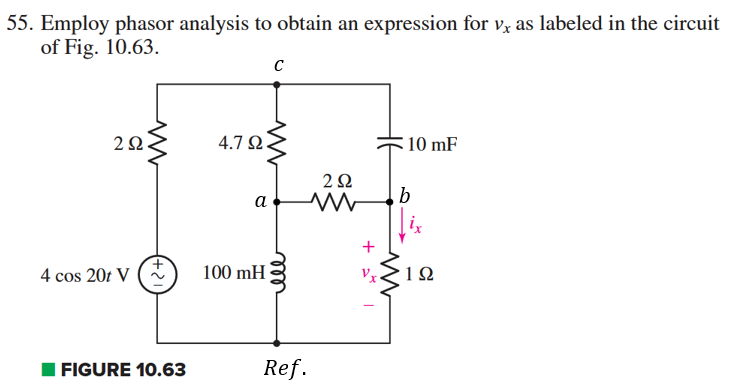
\includegraphics[width=0.8\textwidth]{10-55.png}
\end{center}
Start by putting everything in phasor domain:
\[\mathbf{V_s} = 4\angle 0^\circ\]
Impdences:
\[\frac{1}{j\omega C} = \frac{1}{j[20\,\text{rad/s}]\cdot[10\times10^{-3}\,\text{F}]} = \frac{1}{0.2j} = -5j\]
\[j\omega L = j[20\,\text{rad/s}]\cdot[100\times10^{-3}\,\text{H}] = 2j\]
Using nodal analysis at node c:
\[\frac{\mathbf{V_s}-\mathbf{V_c}}{[2\,\Omega]} = \frac{\mathbf{V_c}-\mathbf{V_a}}{[4.7\,\Omega]}+\frac{\mathbf{V_c}-\mathbf{V_b}}{(-5j)}\]
\[\implies 0.5\mathbf{V_s} = -0.212\mathbf{V_a} + 0.2j\mathbf{V_b}+(0.712+0.2j)\mathbf{V_c}\]
Using nodal analysis at node a:
\[\frac{\mathbf{V_c}-\mathbf{V_a}}{[4.7\,\Omega]}=\frac{\mathbf{V_a}}{(2j)}+\frac{\mathbf{V_a}-\mathbf{V_b}}{[2\,\Omega]}\]
\[\implies 0 = (0.712-0.5j)\mathbf{V_a} - 0.5\mathbf{V_b} - 0.212\mathbf{V_c}\]
Using nodal analysis at node b:
\[\frac{\mathbf{V_c}-\mathbf{V_b}}{(-5j)} + \frac{\mathbf{V_a}-\mathbf{V_b}}{[2\,\Omega]} = \frac{\mathbf{V_b}}{[1\,\Omega]}\]
\[\implies 0 = 0.5\mathbf{V_a} + (-1.5-0.2j)\mathbf{V_b} + 0.2j\mathbf{V_c}\]
Solving this system of equations gives us:
\[\mathbf{V_a} = 0.7031+0.6656j\]
\[\mathbf{V_b} =  0.4093 +0.5627j\]
\[\mathbf{V_c} =  2.9657 -0.7498j\]
Finally, we can find the current through the inductor using $\mathbf{V_b}$. Putting into polar form:
\[\sqrt{(0.4093)^2+(0.5627)^2} = 0.695, \quad \tan^{-1}\left(\frac{0.5627}{0.4093}\right) = 53.96^\circ\]
Thus,
\[\mathbf{V_b} = 0.695\angle 53.96^\circ \implies \boxed{v_x(t) = 0.695\cos(20t + 53.96^\circ)}\]

\section*{10.63}
\vspace{-2em}
\begin{center}
    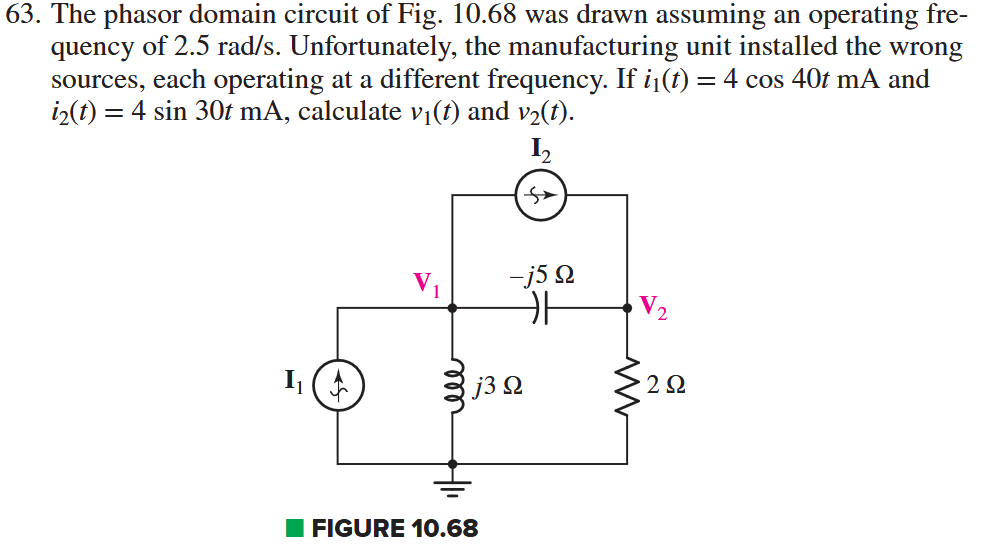
\includegraphics[width=0.8\textwidth]{10-63.png}
\end{center}
Solving for C and L using the given impedances at $\omega = 2.5\,\text{rad/s}$:
\[\frac{1}{j\omega C} = \frac{1}{j[2.5\,\text{rad/s}]\cdot C} = -5j \implies C = 0.08\,\text{F}\]
\[j\omega L = j[2.5\,\text{rad/s}]\cdot L = 3j \implies L = 1.2\,\text{H}\]
Impedances at $\omega = 40\,\text{rad/s}$ ($i_1$):
\[\frac{1}{j\omega C} = \frac{1}{j[40\,\text{rad/s}]\cdot[0.08\,\text{F}]} = \frac{1}{3.2j} = -0.3125j\]
\[j\omega L = j[40\,\text{rad/s}]\cdot[1.2\,\text{H}] = 48j\]
Impedances at $\omega = 30\,\text{rad/s}$ ($i_2$):
\[\frac{1}{j\omega C} = \frac{1}{j[30\,\text{rad/s}]\cdot[0.08\,\text{F}]} = \frac{1}{2.4j} = -0.4167j\]
\[j\omega L = j[30\,\text{rad/s}]\cdot[1.2\,\text{H}] = 36j\]
\textbf{(a)} Using superposition, we start by isolating $i_1$:
\[\mathbf{I_1} = 4\angle 0^\circ\]
Using nodal analysis at node 1:
\[\mathbf{I_1} = \frac{\mathbf{V_1}}{(48j)}+\frac{\mathbf{V_1}-\mathbf{V_2}}{(-0.3125j)}\]
\[\implies \mathbf{I_1} = 3.179j\mathbf{V_1}-3.2j\mathbf{V_2}\]
Using nodal analysis at node 2:
\[\frac{\mathbf{V_1}-\mathbf{V_2}}{(-0.3125j)} = \frac{\mathbf{V_2}}{[2\,\Omega]}\]
\[\implies 0=3.2j\mathbf{V_1}+(-0.5-3.2j)\mathbf{V_2}\]
Solving this system of equations gives us:
\[\mathbf{V_1} = 8.091-0.916j\]
\[\mathbf{V_2} = 8.038+0.339j\]
Convert to polar and find time domain solution:
\[\sqrt{(8.091)^2+(-0.916)^2} = 8.142, \quad \tan^{-1}\left(\frac{-0.916}{8.091}\right) = -6.45^\circ\]
\[\sqrt{(8.038)^2+(0.339)^2} = 8.045, \quad \tan^{-1}\left(\frac{0.339}{8.038}\right) = 2.41^\circ\]
Thus from $i_1$:
\[v_{1,1}(t) = 8.142\cos(40t - 6.45^\circ), \quad v_{2,1}(t) = 8.045\cos(40t + 2.41^\circ)\]
\textbf{(b)} Now isolating $i_2$:
\[\mathbf{I_2} = 4\angle 0^\circ\]
Using nodal analysis at node 1:
\[\frac{\mathbf{V_2}-\mathbf{V_1}}{(-0.4167j)} = \mathbf{I_2} +\frac{\mathbf{V_1}}{(36j)}\]
\[\implies \mathbf{I_2} = -2.37j\mathbf{V_1}+2.39j\mathbf{V_2}\]
Using nodal analysis at node 2:
\[\mathbf{I_2} = \frac{\mathbf{V_2}-\mathbf{V_1}}{(-0.4167j)}+\frac{\mathbf{V_2}}{[2\,\Omega]}\]
\[\implies \mathbf{I_2} = -2.39j\mathbf{V_1}+(0.5+2.39j)\mathbf{V_2}\]
Solving this system of equations gives us:
\[\mathbf{V_1} =  -0.0679+1.685j\]
\[\mathbf{V_2} = -0.0674-0.00271j\]
Convert to polar and find time domain solution:
\[\sqrt{(-0.0679)^2+(1.685)^2} = 1.686, \quad \tan^{-1}\left(\frac{1.685}{-0.0679}\right) = -87.69^\circ\]
Since $\mathbf{V_1}$ is in the second quadrant, we need to add $180^\circ$ to get the correct angle: $\phi = -87.69^\circ + 180^\circ = 92.31^\circ$.
\[\sqrt{(-0.0674)^2+(-0.00271)^2} = 0.0675, \quad \tan^{-1}\left(\frac{-0.00271}{-0.0674}\right) = 2.302^\circ\]
Since $\mathbf{V_2}$ is in the third quadrant, we need to add $180^\circ$ to get the correct angle: $\phi = 2.302^\circ + 180^\circ = 182.3^\circ$.
Thus from $i_2$:
\[v_{1,2}(t) = 1.686\sin(30t + 92.31^\circ), \quad v_{2,2}(t) = 0.0675\sin(30t + 182.3^\circ)\]
Finally, we sum the contributions from $i_1$ and $i_2$ to get the total voltage at each node:
\[\boxed{v_1(t) = v_{1,1}(t) + v_{1,2}(t) = 8.142\cos(40t - 6.45^\circ) + 1.686\sin(30t + 92.31^\circ)\quad\text{[mV]}}\]
\[\boxed{v_2(t) = v_{2,1}(t) + v_{2,2}(t) = 8.045\cos(40t + 2.41^\circ) + 0.0675\sin(30t + 182.3^\circ)\quad\text{[mV]}}\]


\section*{10.66}
\vspace{-2em}
\begin{center}
    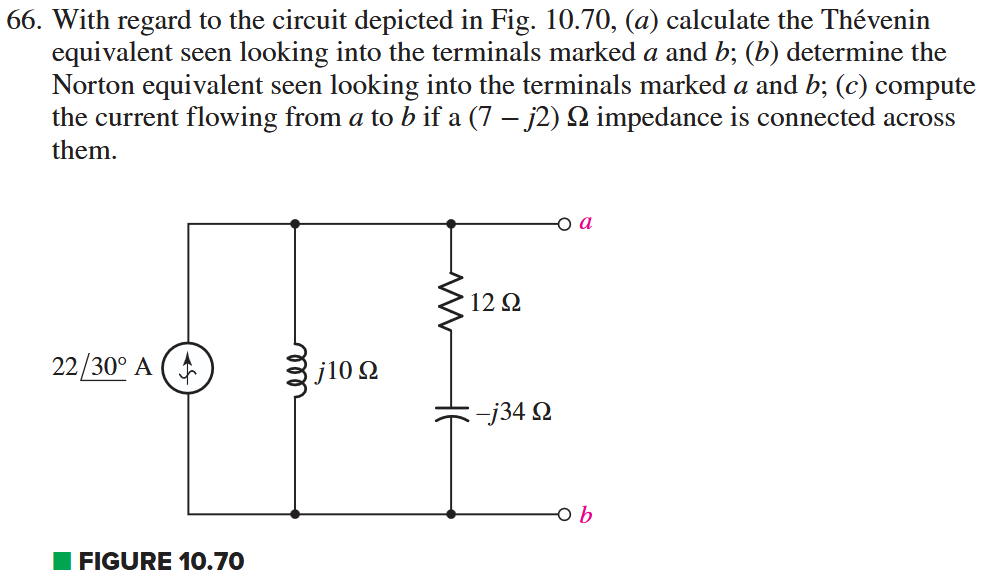
\includegraphics[width=0.8\textwidth]{10-66.png}
\end{center}
\textbf{(a)} Thevennin equivalent circuit:\\\\
Find the equivalent impedance after turning off the source (short circuit for voltage source, open circuit for current source):\\\\
Combine -34j $\Omega$ in series with 12 $\Omega$:
\[\mathbf{Z_1} = -34j + 12\]
Combine $\mathbf{Z_1}$ in parallel with 10j $\Omega$:
\[\mathbf{Z_\text{eq}} = \frac{(12-34j)(10j)}{(12-34j) + 10j}= \frac{120-340j}{12-24j}\]
Convert to polar form to divide:
\[\sqrt{(120)^2+(-340)^2} = 360.55, \quad \tan^{-1}\left(\frac{-340}{120}\right) = -70.56^\circ\quad \text{(numerator)}\]
\[\sqrt{(12)^2+(-24)^2} = 26.83, \quad \tan^{-1}\left(\frac{-24}{12}\right) = -63.43^\circ\quad \text{(denominator)}\]
\[\mathbf{Z_\text{eq}} = \frac{360.55\angle -70.56^\circ}{26.83\angle -63.43^\circ} = 13.44\angle -7.13^\circ\]
Convert back to rectangular form:
\[\boxed{\mathbf{Z_\text{Th}} = \mathbf{Z_\text{eq}} = 13.33 - 1.67j}\]
Find the open circuit voltage $\mathbf{V_{oc}}$:\\\\
The voltage across the parallel branches are all equal to 
\[\mathbf{V} = \mathbf{I_s}\mathbf{Z_\text{eq}} = (22\angle 30^\circ)(13.44\angle -7.13^\circ) = 295.68\angle 22.87^\circ\]
Convert to rectangular form:
\[\boxed{\mathbf{V_{oc}} = 272.5 + 114.2j}\]
\textbf{(b)} Norton equivalent circuit:\\\\
Find the Norton current $\mathbf{I_{N}}$:\\\\
If we short the load (replace with wire), then the current through it is equal to the total source current:
\[\mathbf{I_\text{sc}} = \mathbf{I_s} = 22\angle 30^\circ\]
Convert to rectangular form:
\[\boxed{\mathbf{I_{N}} = 19.05 + 11j}\]
Find the Norton impedance $\mathbf{Z_{N}}$:\\\\
The Norton impedance is the same as the Thevenin impedance:
\[\boxed{\mathbf{Z_{N}} = \mathbf{Z_\text{Th}} = 13.33 - 1.67j}\]
\textbf{(c)} Find current from a to b if (7-2j) $\Omega$ is connected across it:\\\\
Using the Thevenin equivalent circuit, we can use voltage division to find the voltage across the load, and then use $\mathbf{V} = \mathbf{IZ}$ to find the current:
\[\mathbf{V_{ab}} = \frac{(7-2j)}{(7-2j) + (13.33 - 1.67j)}\mathbf{V_{oc}} = \frac{7-2j}{20.33 - 3.67j}\mathbf{V_{oc}}\]
Convert to polar form to divide:
\[\sqrt{(7)^2+(-2)^2} = 7.28, \quad \tan^{-1}\left(\frac{-2}{7}\right) = -15.95^\circ\quad \text{(numerator)}\]
\[\sqrt{(20.33)^2+(-3.67)^2} = 20.66, \quad \tan^{-1}\left(\frac{-3.67}{20.33}\right) = -10.23^\circ\quad \text{(denominator)}\]
\[\mathbf{V_{ab}} = \frac{7.28\angle -15.95^\circ}{20.66\angle -10.23^\circ}\mathbf{V_{oc}} = (0.352\angle -5.72^\circ) \cdot (295.68\angle 22.87^\circ) = 104.1\angle 17.17^\circ\]
Find current:
\[\mathbf{I_{ab}} = \frac{\mathbf{V_{ab}}}{(7-2j)} = \frac{104.1\angle 17.17^\circ}{7.28\angle -15.95^\circ} = 14.3\angle 33.12^\circ\]
Thus,
\[\boxed{i_{ab}(t) = 14.3\cos(100t + 33.12^\circ)\,\text{[A]}}\]

\end{document}